\section[Decay channels]{Radiative and non-radiative decay channels}
\label{sec:TheoDecayChannels}

This section explains why there are multiple ways for the exited state to relax.

As explained in \cref{sec:AbsEmiFlourPhos}, the exited state can transition back to the ground state by emitting a photon. This 
photon carries the energy from the transition. This is called a \textit{radiative decay}.

\begin{figure}[ht]
    \centering
    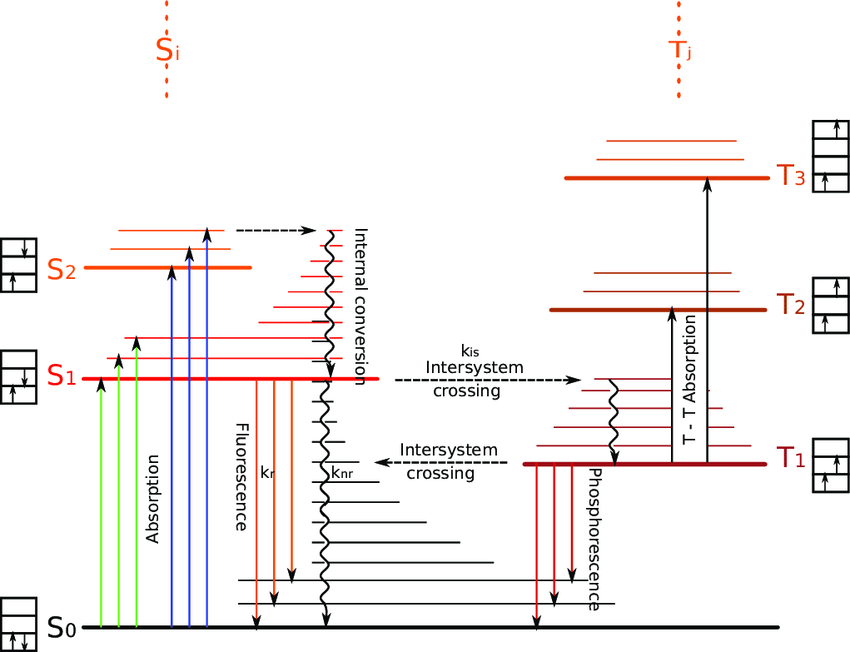
\includegraphics[width = 0.8\textwidth]{Bilder/Grundlagen/Radiative-and-nonradiative-decay-processes-for-systems-obeying-Kashas-rule-Non.png}
    \caption{Radiative and non-radiative decay channels for a single molecule. From \cite{JulienFrancoisGorenflot.2015}}
    \label{fig:DecyChannels}
\end{figure}

In contrast, \textit{non-radiative decay} is the relaxation of an excited state without the emission of light or a photon. It's a process where the excess energy of the excited state is dissipated through other pathways instead of being released as electromagnetic radiation.
There are several mechanisms such as \textit{vibration relaxation, internal conversion, intersystem crossing}, to name a few. In this lab practice intersystem crossing (ISC) will be important. Therefore it is explained briefly.
ISC is a transition that changes the multiplicity of a state. In our case it is the transition from a singlet state $S_{\mathrm{1}}$ to a triplet state $T_{\mathrm{1}}$. This is possible if the
energy level of the state is close. Furthermore, one spin is flipped. This is made possible by spin-orbit-coupling. The two processes are depicted in \cref{fig:DecyChannels}.

The decay of the exited state density $D$ is called the decay rate 

\begin{equation}
    k = \frac{1}{k_{\mathrm{r}}+k_{\mathrm{nr}}}
\end{equation}
where $k_\mathrm{r}$ and $k_{\mathrm{nr}}$ are the radiative and non-radiative decay rate.